% Chapter Template

\chapter{Clean Architecture} % Main chapter title

\label{Chapter5} % Change X to a consecutive number; for referencing this chapter elsewhere, use \ref{ChapterX}

\lhead{Capítulo  5. \emph{Clean Architecture}} % Change X to a consecutive number; this is for the header on each page - perhaps a shortened title

%----------------------------------------------------------------------------------------
%	SECTION 1
%----------------------------------------------------------------------------------------

\section{Modelos de Implementación Clean Architecture}

Los mejores intentos de implementación de esta arquitectura vienen de la mano de un desarrollador argentino Fernando Cejas y los ejemplos de los Blueprints de Google.

\begin{figure}[htbp]
	\centering
	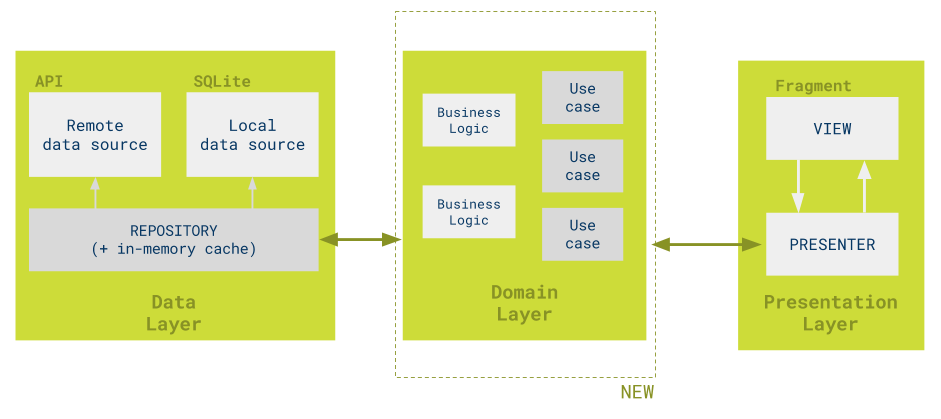
\includegraphics[width=1\textwidth]{Figures/-006.png}
	\rule{35em}{1pt}
	\caption[Principio de Dependecias]{Esquema de dependencias para una arquitectura en capas.}
	\label{fig:Diagrama_clasico}
\end{figure}

Ambas implementaciones están compuestas de tres capas distintas:

\begin{itemize}
	\item Presentation Layer: Esta capa se encarga de interactuar con la UI. Implementa un patrón de diseño conocido como \textbf{MVP (Model View Controller)}. 
	\item Domain Layer: Esta capa contiene toda la lógica de negocio. La capa de dominio comienza con las clases denominadas casos de uso o interactores según la literatura, utilizados por los presentadores de la aplicación. Estos casos de uso representan todas las acciones posibles que un desarrollador puede realizar desde la capa de presentación. Los casos de uso se implementaron utilizando el patrón de diseño conocido como \textbf{Commander}.
	\item Data Layer: Esta capa administra la adquisición de datos y es capaz de utilizar diferentes fuentes de datos. Esta capa se suele implementar utilizando el patrón de diseño conocido como \textbf{Repository}.  
\end{itemize}

\section{Presentation Layer: MVP}
El patrón de arquitectura que se utiliza en la capa de presentación de ambas implementaciones se conoce como Modelo-Vista-Presentador.
La idea detrás del patrón es concentrar la lógica de la interacción con el usuario en una entidad conocida como presentador, las operaciones directamente relacionadas con la manipulación de objetos gráficos y la captura de acciones de usuario están delegadas a la entidad Vista, finalmente la adquisición de datos y la ejecución de los algoritmos que encapsulan la lógica de negocio forman parte de las entidades modelo en el patrón.
El diagrama de componentes que describe la relación entre las partes principales se puede observar a continuación

\begin{figure}[htbp]
	\centering
	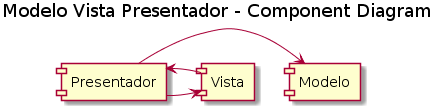
\includegraphics[width=0.7\textwidth]{Figures/uml_mvp_component.png}
	\rule{35em}{1pt}
	\caption[MVP Components]{Diagrama de componentes del patrón.}
	\label{fig:uml_mvp_component}
\end{figure}

Es posible deducir el esquema de comunicación entre los componentes a partir del diagrama. La vista se comunica de manera bidireccional con el presentador y cuando es necesario el presentador se comunica de manera unidireccional con el modelo.


Una convención para la implementación del patrón es tratar de generar vistas completamente ajenas de cualquier lógica operativa y agnósticas del estado de la aplicación. Esto las convierte en un mero instrumento de interfaz entre lo que percibe el usuario y sus reacciones. 

Otra de las convenciones sugiere utilizar objetos modelo-vista en la comunicación entre el presentador y la vista para estandarizar el tipo de mensaje y el proceso de actualización de la vista.

En el caso de las implementaciones antes mencionadas la interfaz con el modelo es satisfecha mediante el uso de objetos casos de uso ó interactores, ambos términos suelen utilizarse de manera intercambiable.

\subsection{Mapeo con Implementaciones}
La capa de presentación tienen una
Una Actividad Android es ejecutada por el proceso principal de la aplicación. La tarea principal de la actividad es inicializar los objetos del patrón: la instancia del fragmento que cumple con el contrato de la vista, la instancia del objeto presentador y las instancias de los casos de uso que serán ejecutados por el presentador.
\begin{itemize}
	\item Vista $\rightarrow$ Fragmento: 
	\item Presentador $\rightarrow$ Presenter
	\item Modelo $\rightarrow$ Casos de Uso
\end{itemize}

El proceso de creación de los objetos y la interacción básica inicial se ilustra en la siguiente diagrama:

\begin{figure}[htbp]
	\centering
	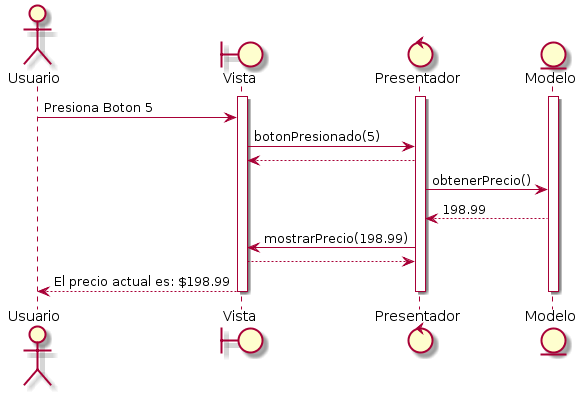
\includegraphics[width=0.7\textwidth]{Figures/uml_mvp_sequence.png}
	\rule{35em}{1pt}
	\caption[MVP Sequence]{Diagrama de secuencia para una interacción con el usuario.}
	\label{fig:uml_mvp_sequence}
\end{figure}

\section{Domain Layer: Commander Pattern}
El patrón de diseño conocido como Commander se utiliza para abstraer la ejecución de procedimientos mediante la implementación de entidades comando. Estos objetos ejecutan un único algoritmo y encapsulan la lógica de negocio de la aplicación o sistema.
Originalmente el diseño contempla 4 entidades principales que se pueden apreciar en el siguiente diagrama de clases:

\begin{figure}[htbp]
	\centering
	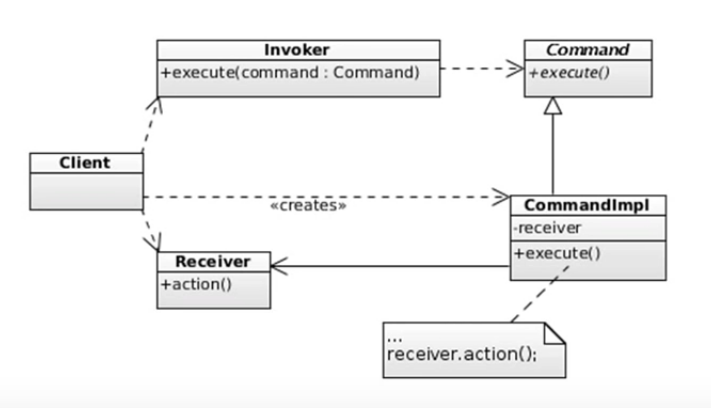
\includegraphics[width=0.7\textwidth]{Figures/uml_clases_commander.png}
	\rule{35em}{1pt}
	\caption[Commander Classes]{Diagrama de clases para el planteo inicial del patrón Commander.}
	\label{fig:uml_clases_commander}
\end{figure}

\begin{enumerate}
	\item Cliente: Este componente se encarga de crear las instancias de cada comando y distribuirlas entre los correspondientes invocadores.
	\item Receptor: Es la entidad que se ve afectada por la ejecución de un comando. Puede ser compartida por varios comandos o bien un único comando puede interactuar con varios receptores en su ejecución.
	\item Comando: Esta entidad contiene la implementación del algoritmo o lógica de ejecución.
	\item Invocador: Se encarga de ejecutar instancias de comandos.
\end{enumerate}

\begin{figure}[htbp]
	\centering
	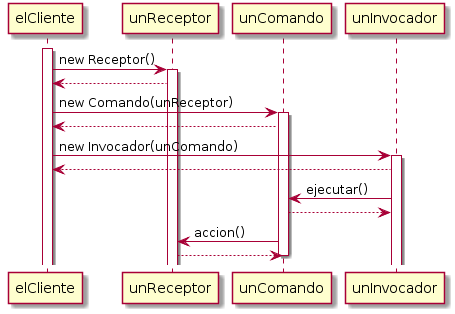
\includegraphics[width=0.7\textwidth]{Figures/uml_sequence_commander.png}
	\rule{35em}{1pt}
	\caption[MVP Components]{Diagrama de secuencia para el patrón Commander.}
	\label{fig:uml_commander_sequence}
\end{figure}

El enfoque inicial sugiere la implementación de un comando
por cada una de las operaciones soportadas por el sistema o aplicación. Sin embargo en sistemas suficientemente grandes la diversidad de funcionalidades soportadas es tan grande que el diseño propuesto se vuelve impráctico.
Para mitigar este problema se suele implementar de manera adicional una modificación que permite la ejecución paramétrica de los comandos para reducir al máximo la cantidad de comandos implementados.
Esta modificación permite diversas alternativas de implementación pero la más utilizada es incorporar conceptos del patrón Request-Response dónde el caso de uso se trata como una entidad de caja negra que admite Solicitudes y emite Respuestas estandarizadas para cada caso.
\begin{itemize}
	\item Solicitud (Request): Un objeto que contiene el conjunto de parámetros de entrada que deben ser satisfechos para poder realizar la ejecución de la rutina del comando.
	\item Respuesta (Response): Un objeto que contiene los valores que se obtuvieron de la ejecución del algoritmo del comando.
\end{itemize}

Por lo tanto puede inferirse el flujo de operación y ejecución de los comandos.

\begin{enumerate}
\item El cliente crea instancias de comandos y sus correspondientes invocadores. 
\item El invocador crea e inicializa los objeto solicitud necesarios para ejecutar cada comando.
\item El invocado ejecuta los comandos llamando al método ''ejecutar'' implementado por cada comando pasando como parámetro la solicitud previamente creada.
\item El invocador observa los resultados en espera activa implementando el patrón Observer o mediante algún esquema de callback.
\end{enumerate}

\begin{figure}[htbp]
	\centering
	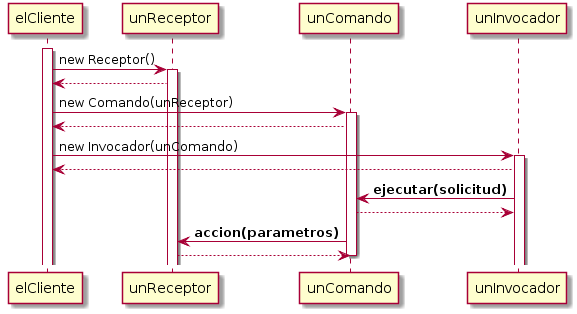
\includegraphics[width=0.8\textwidth]{Figures/uml_sequence_commander_req_resp.png}
	\rule{35em}{1pt}
	\caption[Commander Review]{Diagrama de secuencia para el diseño revisado.}
	\label{fig:uml_commander_sequence_req_resp}
\end{figure}

Siguiendo los lineamientos de la arquitectura propuesta los autores denominan a los comandos: Casos de Uso, ó Interactores.

En las implementaciones estudiadas se encontraron las correspondencias como se listan a continuación:
\begin{itemize}
	\item Cliente $\rightarrow$ Actividad
	\item Receptor $\rightarrow$ Repositorio
	\item Comando $\rightarrow$ CasoDeUso
	\item Invocador $\rightarrow$ Presentador
\end{itemize}

Como una nota relevante de implementación se recomienda ejecutar las rutinas de los comandos en un hilo/proceso separado para para evitar bloquear el proceso principal de la aplicación.



\section{Data Layer: Repository Pattern}
En la capa de datos se propone la implementación de un patrón de diseño conocido como Repository(Repositorio). 
Originalmente se concibe a este diseño como una forma de estandarizar la implementación y el uso de los objetos DAO (Data Access Object) comúnmente utilizados para mapear objetos entidad con las persistencias en la base de datos.
Adicionalmente este patrón encapsula en la clase repositorio todos los métodos particulares de filtrado, procesamiento calculado y ordenamiento de entidades.
Sin embargo se define una interfaz genérica que deberá ser respetada por todas las implementaciones de repositorios para todo el sistema independientemente de la entidad que atienda.

\begin{figure}[htbp]
	\centering
	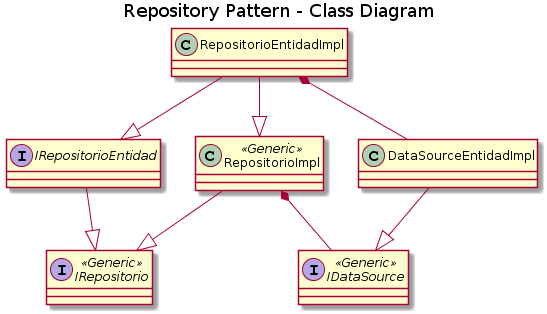
\includegraphics[width=0.8\textwidth]{Figures/uml_clases_repository.png}
	\rule{35em}{1pt}
	\caption[Repository Pattern Class Diagram]{Diagrama de clases del patrón Repository.}
	\label{fig:uml_clases_repository}
\end{figure}

Como puede apreciarse en el diagrama se definen:
\begin{itemize}
	\item IRepositorio: es una interfaz genérica que establece el contrato básico que deben respetar todas las implementaciones de repositorios.
	\item RepositorioImpl: es una clase genérica que establece la interacción con una fuente de datos genérica.
	\item IRepositorioEntidad: es la interfaz que \textit{Especifica} la interfaz genérica de repositorio y establece el contrato o métodos particulares que deberá cumplir la implementación concreta de repositorio para esta Entidad en particular.
	\item RepositorioEntidadImpl: es la clase que \textit{Especifica} la implementación genérica de repositorio e implementa los métodos particulares para esta Entidad en particular.
\end{itemize}

En una descripción más detallada del diagrama puede observarse que existen dos interfaces genéricas para acceso de datos IRepository y IDataSource, esto podría generar confusión y ser de alguna forma repetitivo.

\begin{figure}[htbp]
	\centering
	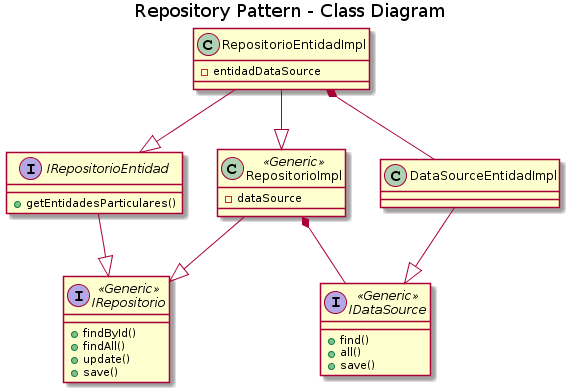
\includegraphics[width=0.8\textwidth]{Figures/uml_clases_detalles_repository.png}
	\rule{35em}{1pt}
	\caption[Repository Pattern Detailed Class Diagram]{Diagrama de clases detallado del patrón Repository.}
	\label{fig:uml_clases_detalles_repository}
\end{figure}

 Por lo antes expuesto parece razonable plantear una fusión entre el concepto de repositorio y fuente de datos. Coloquialmente es trivial ya que un repositorio definitivamente es una fuente de datos. Si además se quita la estandarización por genéricos se consigue un diseño más flexible.
 
 \begin{figure}[htbp]
 	\centering
 	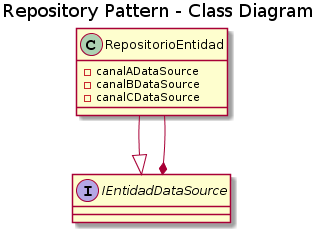
\includegraphics[width=0.5\textwidth]{Figures/uml_clases_modif_repository.png}
 	\rule{35em}{1pt}
 	\caption[Modified Repository Pattern Class Diagram]{Diagrama de clases del patrón Repository modificado.}
 	\label{fig:uml_clases_modif_repository}
 \end{figure}

Principalmente orientado a encapsular la manipulación, selección, priorización y mantenimiento de diversas fuentes u orígenes de datos, este esquema de repositorios modificado permite que el peticionario se comunique con una única interfaz para solicitar operaciones sobre datos permaneciendo agnóstico del origen de datos sobre el cual tendrán impacto. 
Implementar una política de caching local se convierte en una tarea sencilla de implementar y mantener.
Esta es la implementación del patrón que se observó en los códigos estudiados.
% 
